\documentclass[12pt]{article}

\title{\vspace{-3em}164a HW 1}
\author{Michael Cardiff}
\date{\today}

%% science symbols 
\usepackage{amsmath}
\usepackage{amssymb}
\usepackage{physics}
\usepackage{slashed}
\usepackage{siunitx}

%% general pretty stuff
\usepackage{bm}
\usepackage{enumitem}
\usepackage{float}
\usepackage{graphicx}
\usepackage[margin=1in]{geometry}
\usepackage[labelfont=bf]{caption}

% figures

\newcommand{\fig}[3]
{
  \begin{figure}[H]
    \centering
    \includegraphics[width=#1cm]{#2}
    \caption{#3}
  \end{figure}
}

\newcommand{\figref}[4]
{
  \begin{figure}[H]
    \centering
    \includegraphics[width=#1cm]{#2}
    \caption{#3}
    \label{#4}
  \end{figure}
}

\renewcommand{\L}{\mathcal{L}}
\newcommand{\D}{\partial}
\newcommand{\munu}{{\mu\nu}}
\newcommand{\sla}[1]{\slashed{#1}}

\begin{document}
\maketitle
\section{Masses}
\begin{table}[H]
  \centering
  \begin{tabular}{c|c|c}
    Object & (kg) & (GeV) \\\hline
    Proton           & \num{1.6e-27} & \num{9.38e-1} \\
    Hydrogen Atom    & \num{1.7e-27} & \num{9.4e-1} \\
    Carbon Atom      & \num{2.0e-26} & \num{6.7e1} \\
    Bacterium        & \num{1.0e-15} & \num{5.6e11} \\
    Blood Cell       & \num{2.7e-14} & \num{1.5e13} \\
    People           & \num{6.2e1  }   & \num{3.4e28} \\
    Antartic Whale   & \num{1.8e5  }   & \num{1.0e32} \\
    Moon             & \num{7.3e22 }  & \num{4.1e49} \\
    Earth            & \num{5.9e24 }  & \num{3.3e51} \\
    Sun              & \num{1.9e30 }  & \num{1.1e57} \\
    Solar System     & \num{2.0e30 }  & \num{1.12e57} \\
    Milky Way Galaxy & \num{2.9e42 }  & \num{1.6e69}
  \end{tabular}
  \caption{Masses of the objects}
\end{table}

\section{Sizes}

\begin{table}[H]
  \centering
  \begin{tabular}{c|c|c}
    Object & (m) & (ft) \\\hline
    Proton           & \num{8.4e-16} & \num{2.8e-15} \\
    Hydrogen Atom    & \num{1.2e-10} & \num{3.9e-10} \\
    Carbon Atom      & \num{1.7e-10} & \num{5.6e-10} \\
    Bacterium        & \num{1.1e-6}  & \num{3.6e-6 } \\
    Blood Cell       & \num{3.8e-6}  & \num{1.2e-5 } \\
    People           & \num{1.6e1}   & \num{5.2e0  } \\
    Antartic Whale   & \num{2.0e1}   & \num{6.6e1  } \\
    Moon             & \num{1.7e6}   & \num{5.6e6  } \\
    Earth            & \num{6.4e6}   & \num{2.1e7  } \\
    Sun              & \num{7.0e8}   & \num{2.3e9  } \\
    Solar System     & \num{1.4e14}  & \num{3.6e14 } \\
    Milky Way Galaxy & \num{5.0e20}  & \num{1.6e+21}
  \end{tabular}
  \caption{Sizes of the objects}
\end{table}
\newpage
\section{Plots}

These are the plots created, using a python script to fit and plot the data:
\begin{figure}[H]
  \centering
  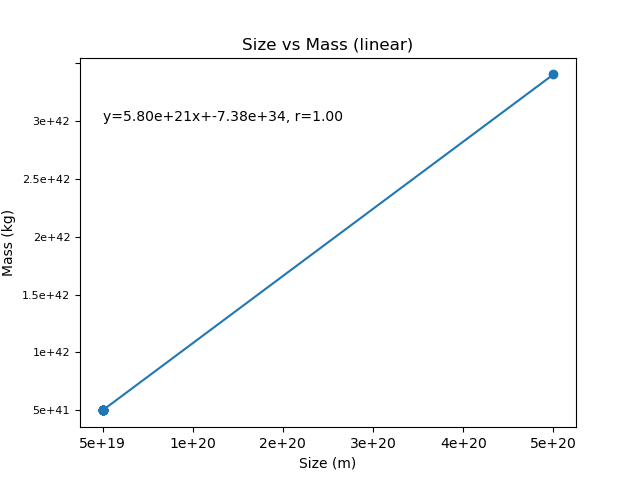
\includegraphics[width=12.0cm]{linear}
  \caption{The linear plot}
  \label{fig:1}
\end{figure}
\begin{figure}[H]
  \centering
  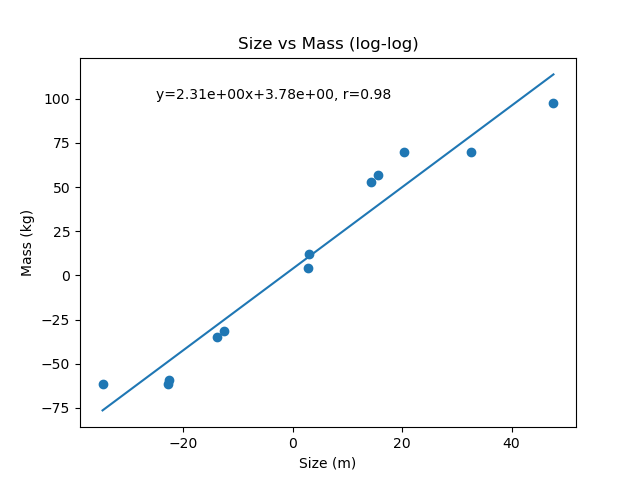
\includegraphics[width=12.0cm]{loglog}
  \caption{The log-log plot}
  \label{fig:2}
\end{figure}
The fit coefficient for the linear plot is 1.0, and for the log-log plot it is 0.98

The equation for the linear fit:
\begin{equation*}
  y = \num{5.80e21}x+\num{7.8e34}
\end{equation*}
For the log-log fit:
\begin{equation*}
  y = 2.31x+3.78
\end{equation*}
The log-log fit is clearly the more useful of the 2, giving a sense of how each of these parameters change with a sense of order of magnitude rather than how they change by pure value. This is infinitely more useful in physics as the span of objects which different fields of physics describe spans hundreds of orders of magnitude.

The uselessness of the linear plot comes mostly from not only the relative small sizes and masses of the objects on the lower end, but also the relatively large sizes and masses of the largest objects. If we were to group the objects by similar orders of magnitude and plotted those individually, the plots would look a lot better without needing to use a log-log. This is best seen with the fit coefficient in the linear plot. While it is calculated as 1.0, this can surely be attributed to the sheer span of the dataset which is being considered
\end{document}